\chapter{Distribute Concurrency Control}

Distributed concurrency control ensures the correct execution of operations that affect data that are
stored in a distributed fashion on different database servers.

Specifications of concurrency control protocols use the term \textbf{agent} for each stakeholder participating to the protocol.
\begin{itemize}
    \item Each agent can furthermore have different \textbf{roles}
    \item The most important is the \textbf{coordinator} which is the database server that communicates with all other agents
    \item Concurrency protocols hence offer a solution to the \textbf{consensus problem}: the consensus problem requires a set of agents to agree on a single value.
\end{itemize}

\begin{tcolorbox}
\begin{itemize}
    \item The \textbf{two-phase commit}requires \textit{all participating} agents to agree to a proposed value in order to accept the value as the currently globally valid state among all agents
    \item In contrast, \textbf{quorum consensus} protocols only require a certain \textit{majority} of agents to agree on a proposed value
    \item The \textbf{Paxos algorithm} as a prominent and widely used quorum consensus protocol
    \item Lastly, \textbf{multi-version concurrency control} as a timestamp based concurrency mechanism that offers non-blocking reads
\end{itemize}
\end{tcolorbox}

\section{Two-Phase Commit}
\begin{itemize}
    \item The two-phase commit (2PC) addresses the execution of a \textit{distributed transaction} where all agents have to acknowledge a successful finalization of the transaction
    \item 2PC is initiated by the coordinator of the transaction who wants to reach a consensus
    \item In the simplest case, all agents try to agree on accepting a single value of an update request that has been received by the coordinator
\end{itemize}
\newpage
It has two phases: \textbf{voting phase} and a \textbf{decision phase}:
\begin{figure}[h!]
\centering
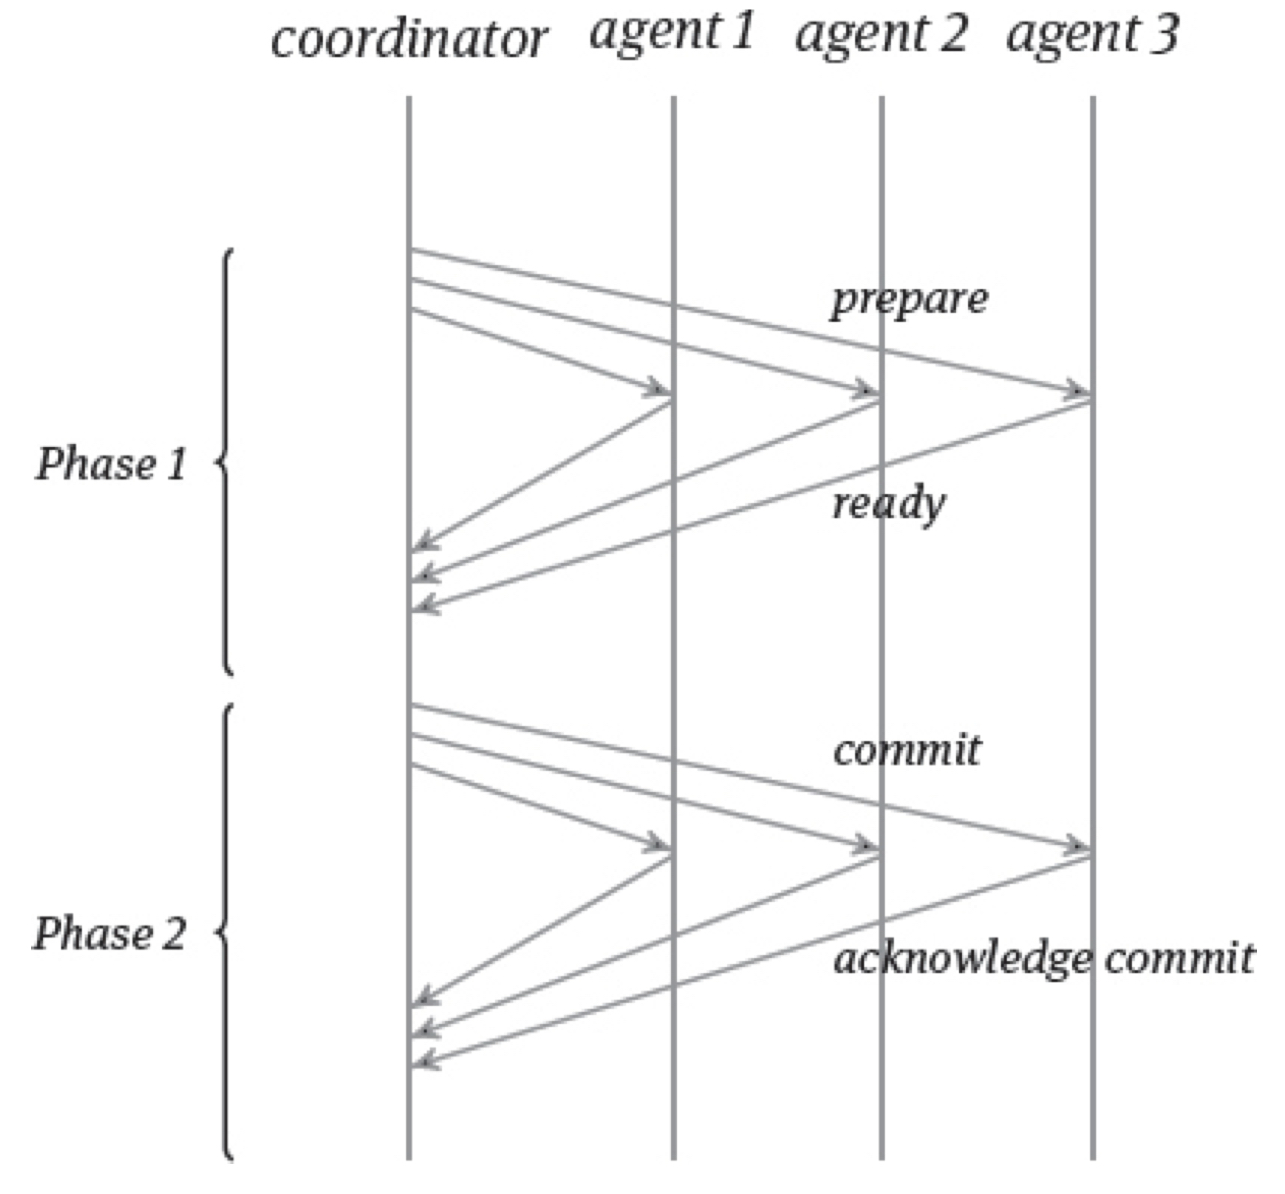
\includegraphics[width=.5\linewidth]{images/AdvancedDataManagment/distribute_concurrency_control/2pc-commit_case.jpeg}
\end{figure}

\begin{itemize}
    \item In each phase, the coordinator sends one message to all agents and receives a reply from each agent
    \item In case no timeouts and no restarts occur, the agents can either jointly agree to commit the value or the coordinator decides to abort the transaction
    \item \textbf{Voting phase:} the coordinator sends all agents a \textbf{prepare} message asking f they can commit the transaction. Each agent can:
    \begin{itemize}
        \item Replay \textit{ready}
        \item Replay \textit{failed}
        \item Do not replay, causing the time out protocol handling this case
    \end{itemize}
    \item \textbf{Decision phase}, the coordinator notifies the agents of a common decision resulting from the votes: 
    \begin{itemize}
        \item The transaction can only be \textbf{globally committed} if all agents voted \textit{ready} in which case the coordinator sends a commit message to all agents
        \item The \textbf{abort} case applies if at least one agent voted \textit{failed}. In order
        to abort the transaction globally, the coordinator has to send an \textit{abort message} to all agents that have voted \textit{ready}
    \end{itemize}
\end{itemize}

\begin{tcolorbox}
A major problem is that a failure of a single agent will lead to a global abort of the transaction. Moreover, the protocol highly depends on the central role of a single coordinator. In particular, the state between the two phases is called the \textbf{in-doubt state}:

\begin{itemize}
    \item In case the coordinator irrecoverably fails before sending his decision, the agents cannot proceed to either commit or abort the transaction
    \item It can only be solved by a complex recovery procedure that contacts all other agents and asks for their votes again
\end{itemize}
\end{tcolorbox}

\begin{figure}[h!]
\centering
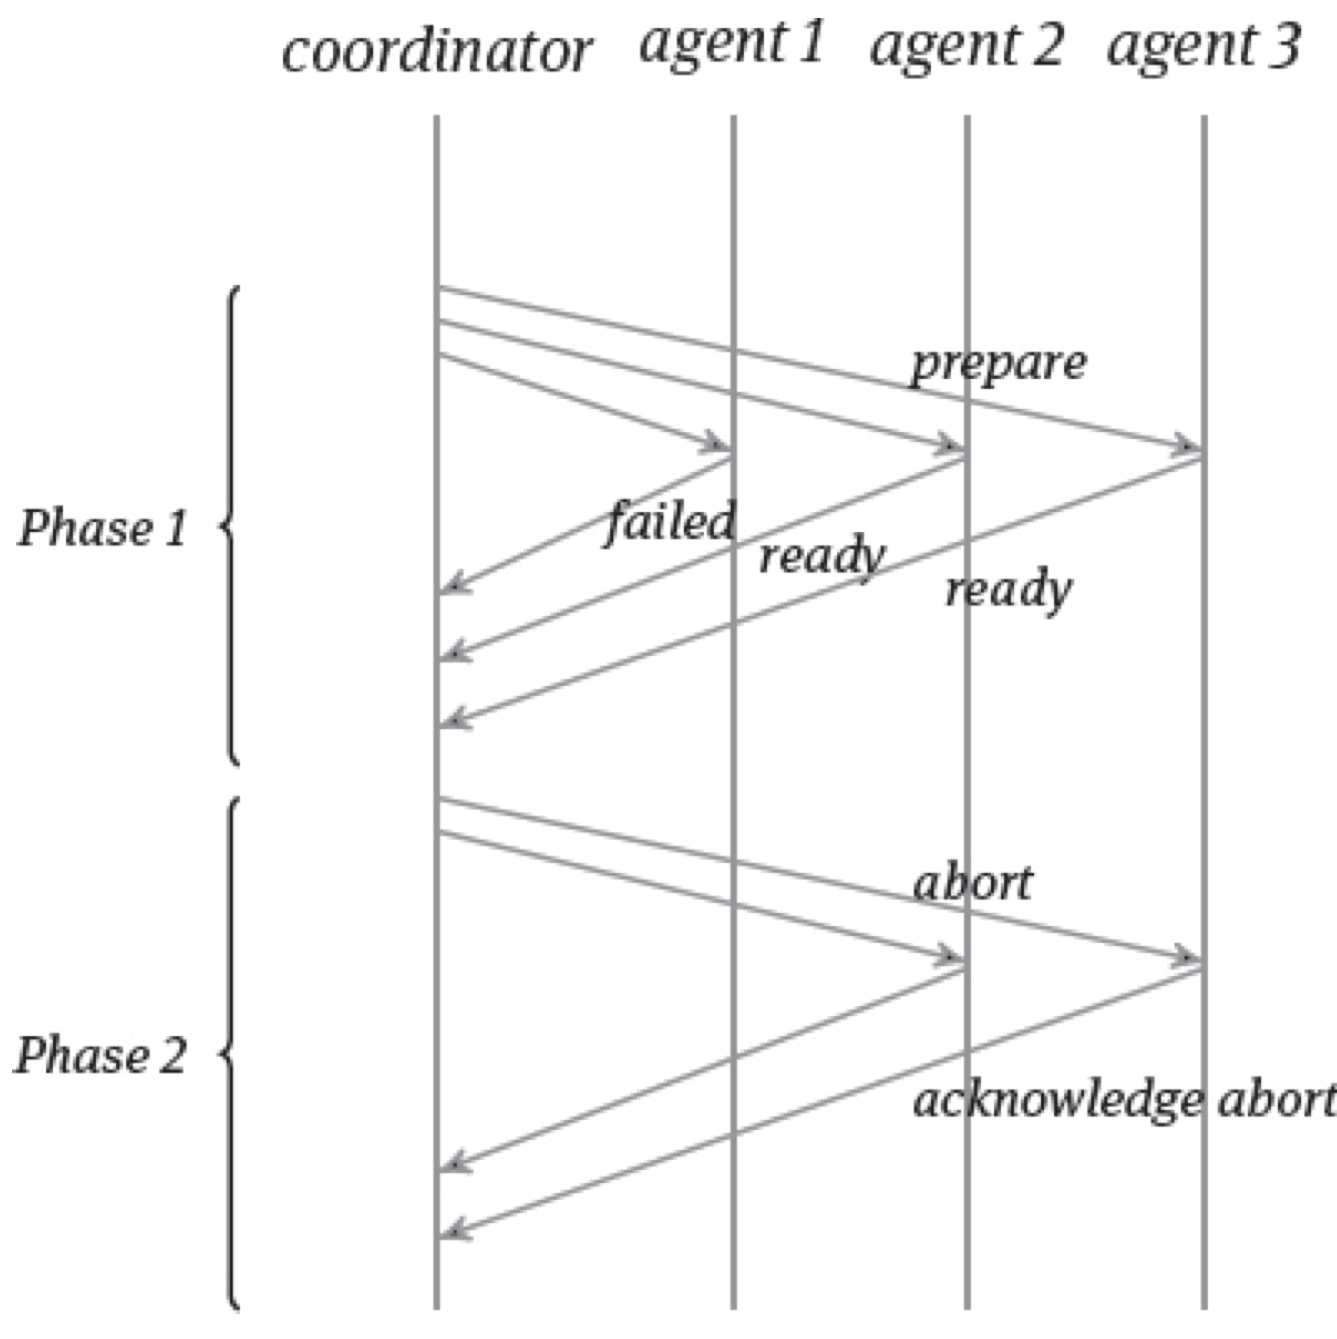
\includegraphics[width=.5\linewidth]{images/AdvancedDataManagment/distribute_concurrency_control/2pc-abort_case.jpeg}
\end{figure}

A so-called three-phase commit protocol adds another phase (the pre-commit phase) to avoid this blocking behavior

\section{Pasox Algorithm}
The basic Paxos algorithm is meant to cope with non-Byzantine failures and it can be applied to keep a distributed DBMS in a consistent state.

A client can for example issue a read request for some database record; the database servers then have to come to a consensus on what the current state of the record is.

The following types of agents take part in a Paxos protocol:
\begin{itemize}
    \item \textbf{Proposer:} 
    \begin{itemize}
        \item A proposer is an agent that waits for a client request and then initiates the consensus process
        \item A proposer assigns a number to its request
        \item Depending on the answers received from the acceptors, the proposer chooses a response value
    \end{itemize}
    \item \textbf{Leader:} for handling a specific client request, one of the proposers is elected to be the leader
    \item \textbf{Acceptor:} 
    \begin{itemize}
        \item An acceptor can accept a proposal based on the proposed value and on the proposal number
        \item Correct acceptor only accepts proposals which are numbered higher than any proposal it has accepted before
        \item So acceptor has to always remember the highest proposal it accepted so far
    \end{itemize}
    \item \textbf{Learner:}
    \begin{itemize}
        \item Is any other agent that is interested in the value on which the acceptors agreed
        \item Learners will be informed of a response value by each of the acceptors
        \item Usually, the leader is also a learner so that he receives the notification that his chosen value was finally agreed to by a majority of acceptors
    \end{itemize}
\end{itemize}

\begin{figure}[h!]
\centering
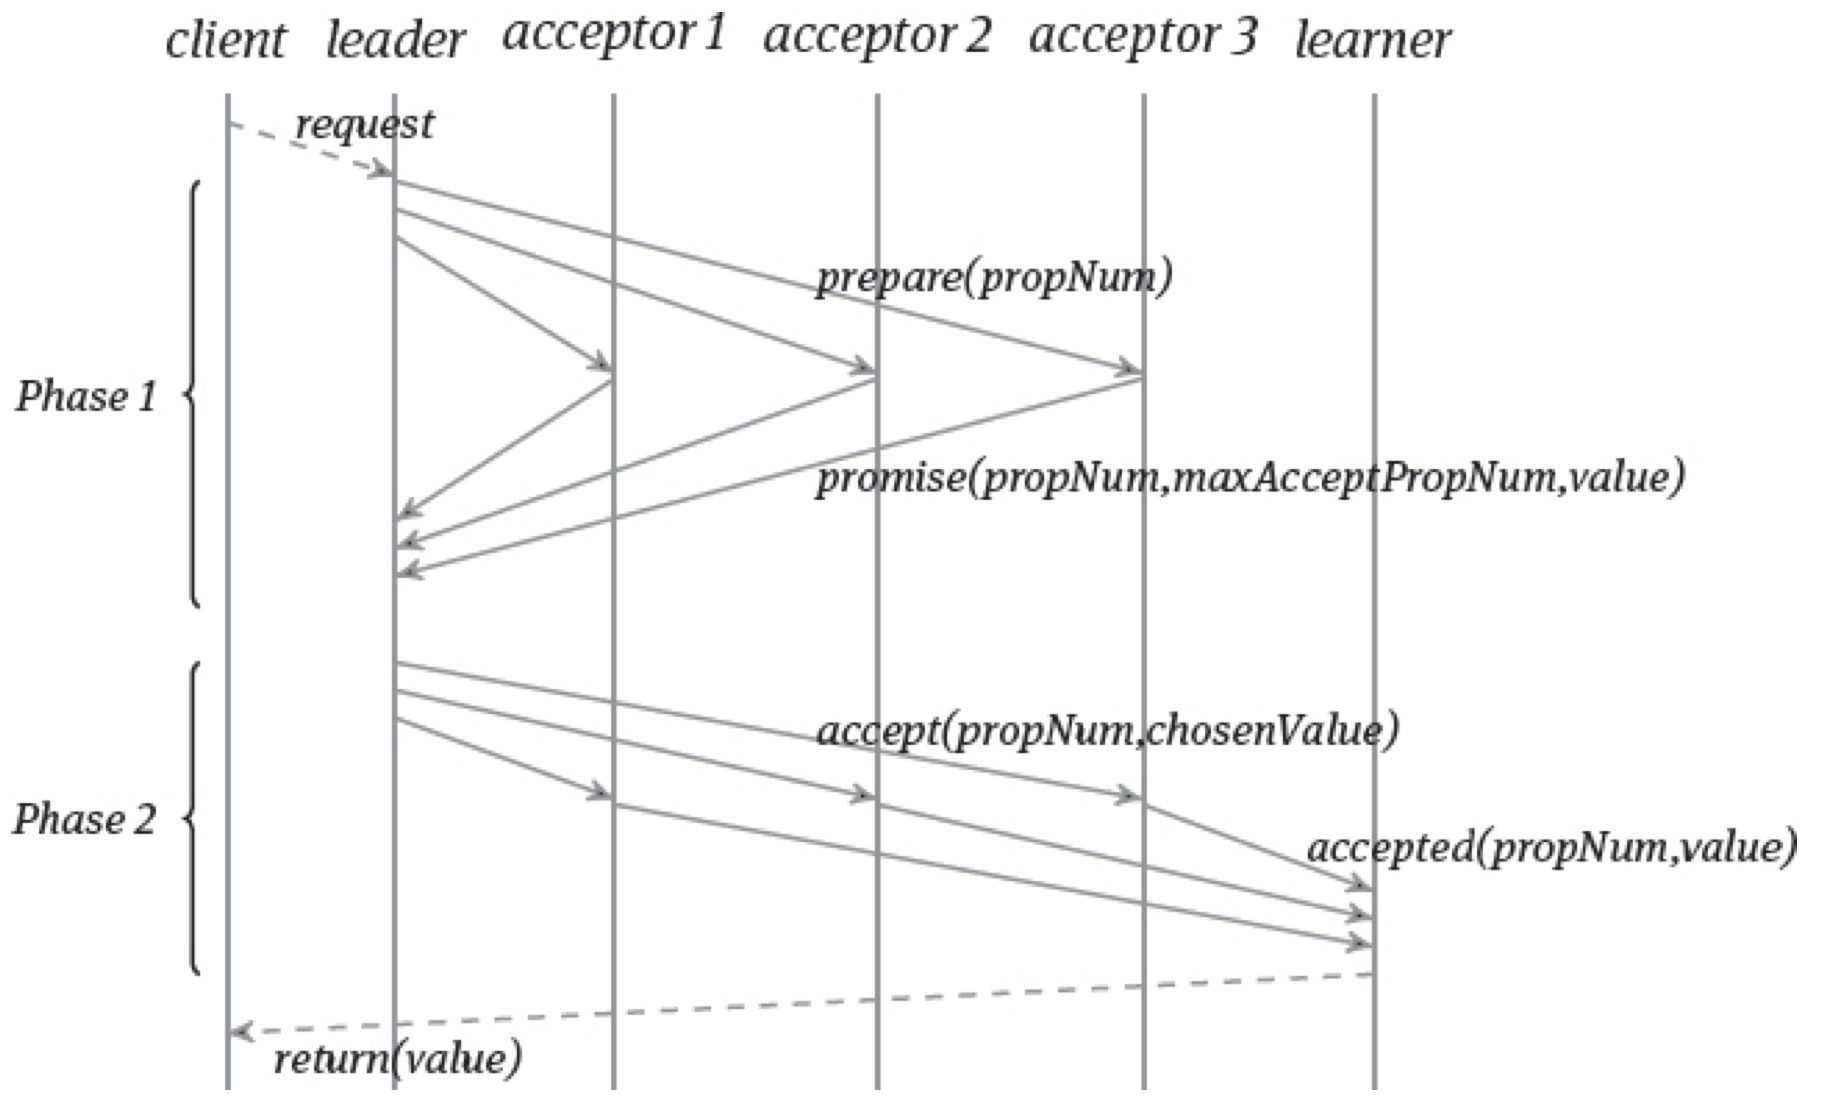
\includegraphics[width=.7\linewidth]{images/AdvancedDataManagment/distribute_concurrency_control/pasox.jpeg}
\end{figure}

With the basic Paxos protocol the following safety properties are guaranteed to hold for each individual run of the protocol:
\begin{itemize}
    \item \textbf{Nontriviality:} Any value that a learner learns must have been proposed by a proposer
    \item \textbf{Stability:} A learner learns one single value or none at all
    \item \textbf{Consistency:} All learners learn the same value
    \item \textbf{Liveness:} If some value has been proposed, a learner will learn a value
\end{itemize}

The basic Paxos protocol can support non-Byzantine failures of the participating agents as follows:
\begin{itemize}
    \item \textbf{Failures of proposers:} The leader can fail as long as there is at least one backup proposer who can be the new leader and eventually gets his chosen value accepted
    \item \textbf{Failures of learners:} If all learners fail, the consensus value will not be sent to the client although a majority of acceptors accepted a chosen value. Hence, there must be at least one learner working correctly
    \item \textbf{Failures of acceptors:} The leader has to receive promise messages for the proposal number from a majority of acceptors and later on at least one learner has to receive accepted messages for the proposal number from a majority of acceptors
\end{itemize}
If however a majority of acceptors fails, a new run of Phase 1 has to be started with a higher proposal number and with a quorum containing other acceptors than the failed ones.

\section{Vector Clock}
The strong clock property is satisfied for \textbf{vector clocks}: a vector clock is a vector of counters with one counter for each client process. With vector clocks it is crucial to have a separate counter for each client processes as otherwise servers could not accept concurrent write requests from multiple users.

\section{Version Vectors}
\begin{tcolorbox}
While vector clocks are a mechanism for stepping forward the time in a messagepassing system, version vectors are a mechanism to consolidate and synchronize several replicas of a data record.
\end{tcolorbox}
\begin{itemize}
    \item In order to determine which view of the state of the database contents each user has, for every read request for a data record the answer contains the current version vector for that data record
    \item When subsequently the user writes that same data record, the most recently read version vector is sent with the write request as the so called \textbf{context}
    \item With this context, the database system can decide how to order or merge the writes
    \item Conflicting versions can for example occur with multi-master replication, this is the case of conflicting writes
    \item A \textbf{synchronization} process reconciles conflicting replicas
    \item A simple form of synchronization of two conflicting replicas is to take the \textit{union} of them
    \item The process of maintaining version vectors is slightly different from the one for maintaining vector clocks. The aim is to reconcile divergent replicas into one common version
\end{itemize}


We now describe version vector maintenance with \textbf{union semantics} for the synchronization process. In this setting, each data record consists of a set of values and the synchronization of the data record computes the set union; that is, the result of a merge is again a set of values. And it is composed by the following steps:
\begin{enumerate}
    \item \textbf{Initialization:}
    \begin{itemize}
        \item For \textbf{n} client processes, a version vector is a vector of \textbf{n} elements
        \item Each replica of a data record maintains one version vector
        \item Initially, for each process all elements are 0
    \end{itemize}
    \item \textbf{Update:}
    \begin{itemize}
        \item When a client process j sends a write request to overwrite a set of values at replica i, it sends the new set of values and the context
        \item Based on the context, it decide to overwrite its value set or take the union
        \item Then computes the maximum over the context and its own version vector
    \end{itemize}
    \item \textbf{Synchronization:}
    \begin{itemize}
        \item Whenever two replicas i and j have different version vectors
        \item The synchronization process reconciles the two versions by either overwriting one value set or by taking the union of the two value sets
    \end{itemize}
\end{enumerate}

\begin{figure}[h!]
\centering
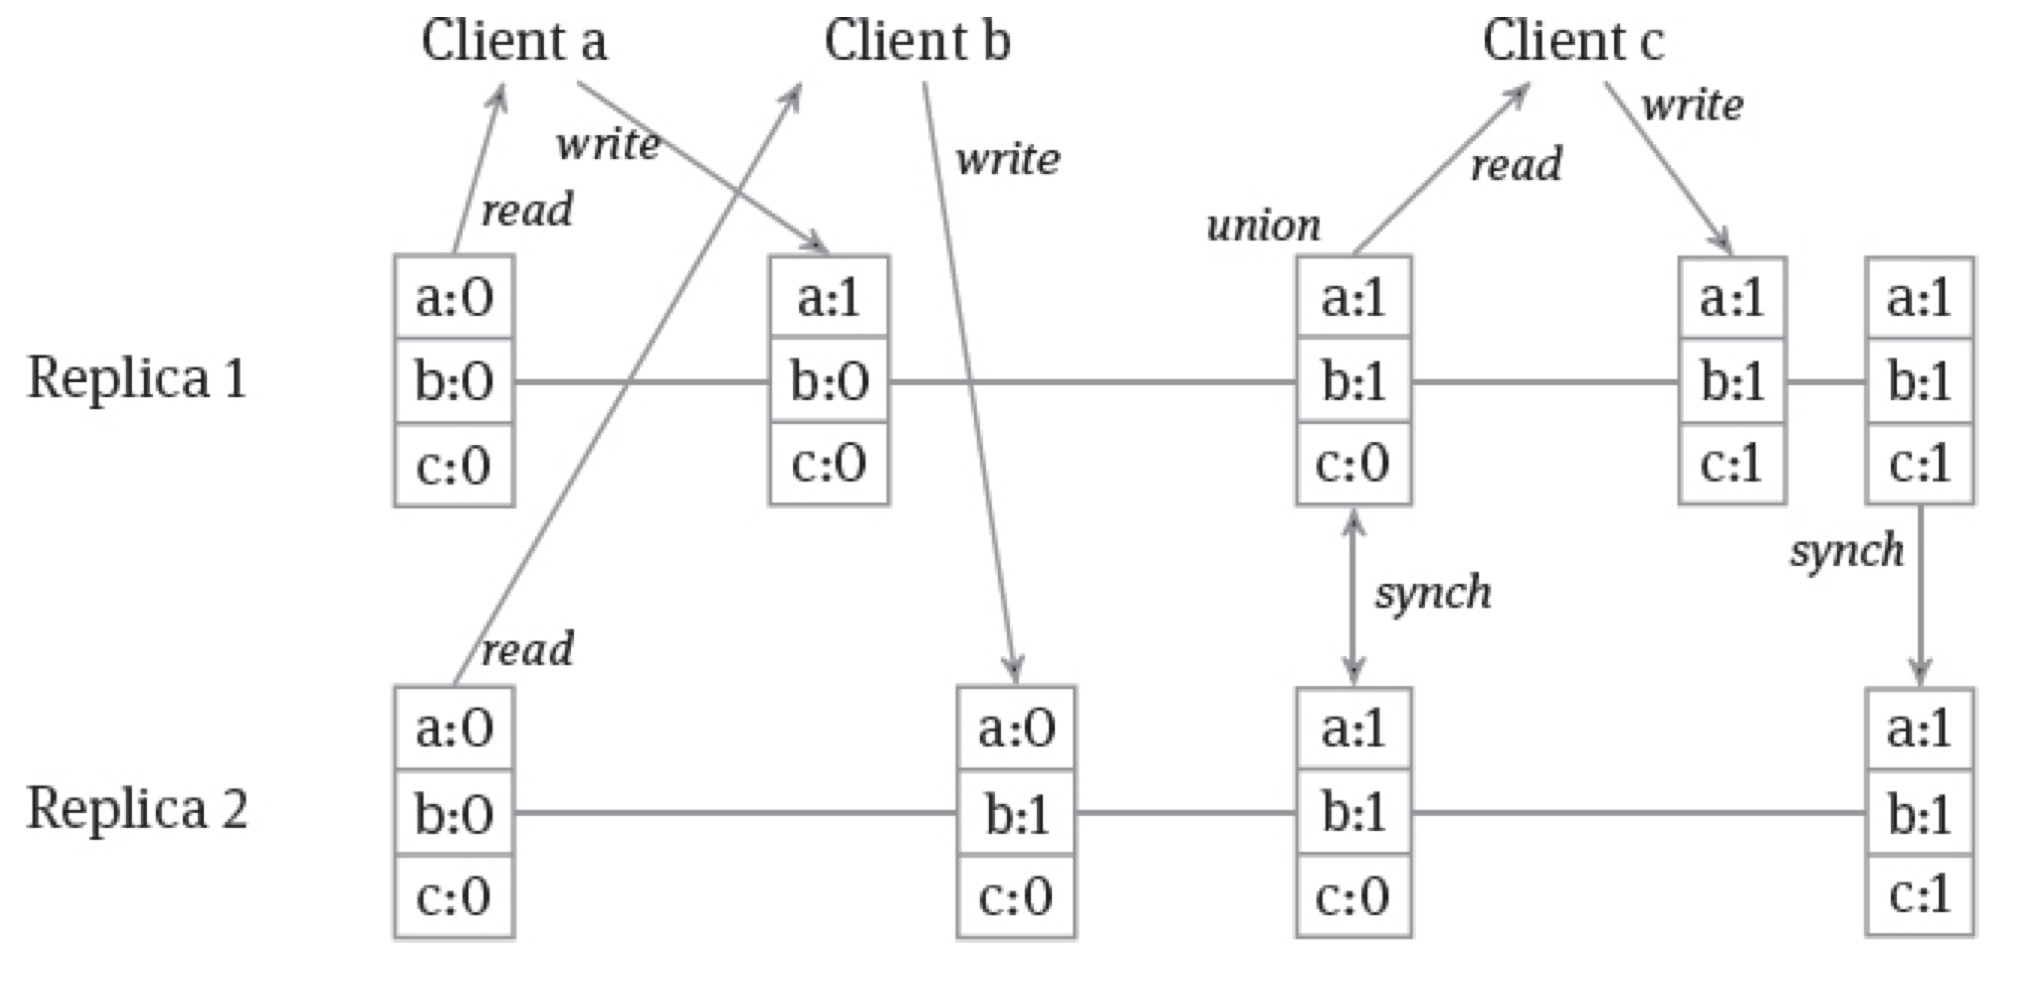
\includegraphics[width=.7\linewidth]{images/AdvancedDataManagment/distribute_concurrency_control/version_vector-union_merge.jpeg}
\end{figure}



More advanced forms of merging usually involve a semantic decision that requires interaction of the user or a more intelligent application logic. If such a user interaction is needed, \textbf{sibling versions} for a data record have to be maintained until the user writes a merged version:
\begin{itemize}
    \item The database systems stores all concurrent versions together with their attached version vectors
    \item As soon as a user writes a merged version that is meant to replace the siblings, the version vector of the merged version is set to be larger than all the version vectors of the siblings
    \item And then the siblings can be deleted
\end{itemize}

More formally, version vector maintenance with sibling semantics works as follows:
\begin{enumerate}
    \item \textbf{Initialization:}
    \begin{itemize}
        \item For \textbf{n} client processes, a version vector is a vector of \textbf{n} elements
        \item Each replica of a data record maintains a set D of pairs of values and version vectors
    \end{itemize}
    \item \textbf{Update:}
    \begin{itemize}
        \item When a client process $j$ sends a write request to overwrite some or all values in the data set $D_i$ at replica $i$, it sends the new value $val_j$ and the context $C_j$
        \item The replica checks which siblings in $D_i$ are covered by $C_j$, then computes the maximum over the context
    \end{itemize}
    \item \textbf{Synchronization:}
    \begin{itemize}
        \item Whenever two replicas $i$ and $j$ have different data sets $D_i$ and $D_j$ for one data record, the synchronization process reconciles the two versions by only keeping the values with the highest version vectors
    \end{itemize}
\end{enumerate}


\begin{figure}[h!]
\centering
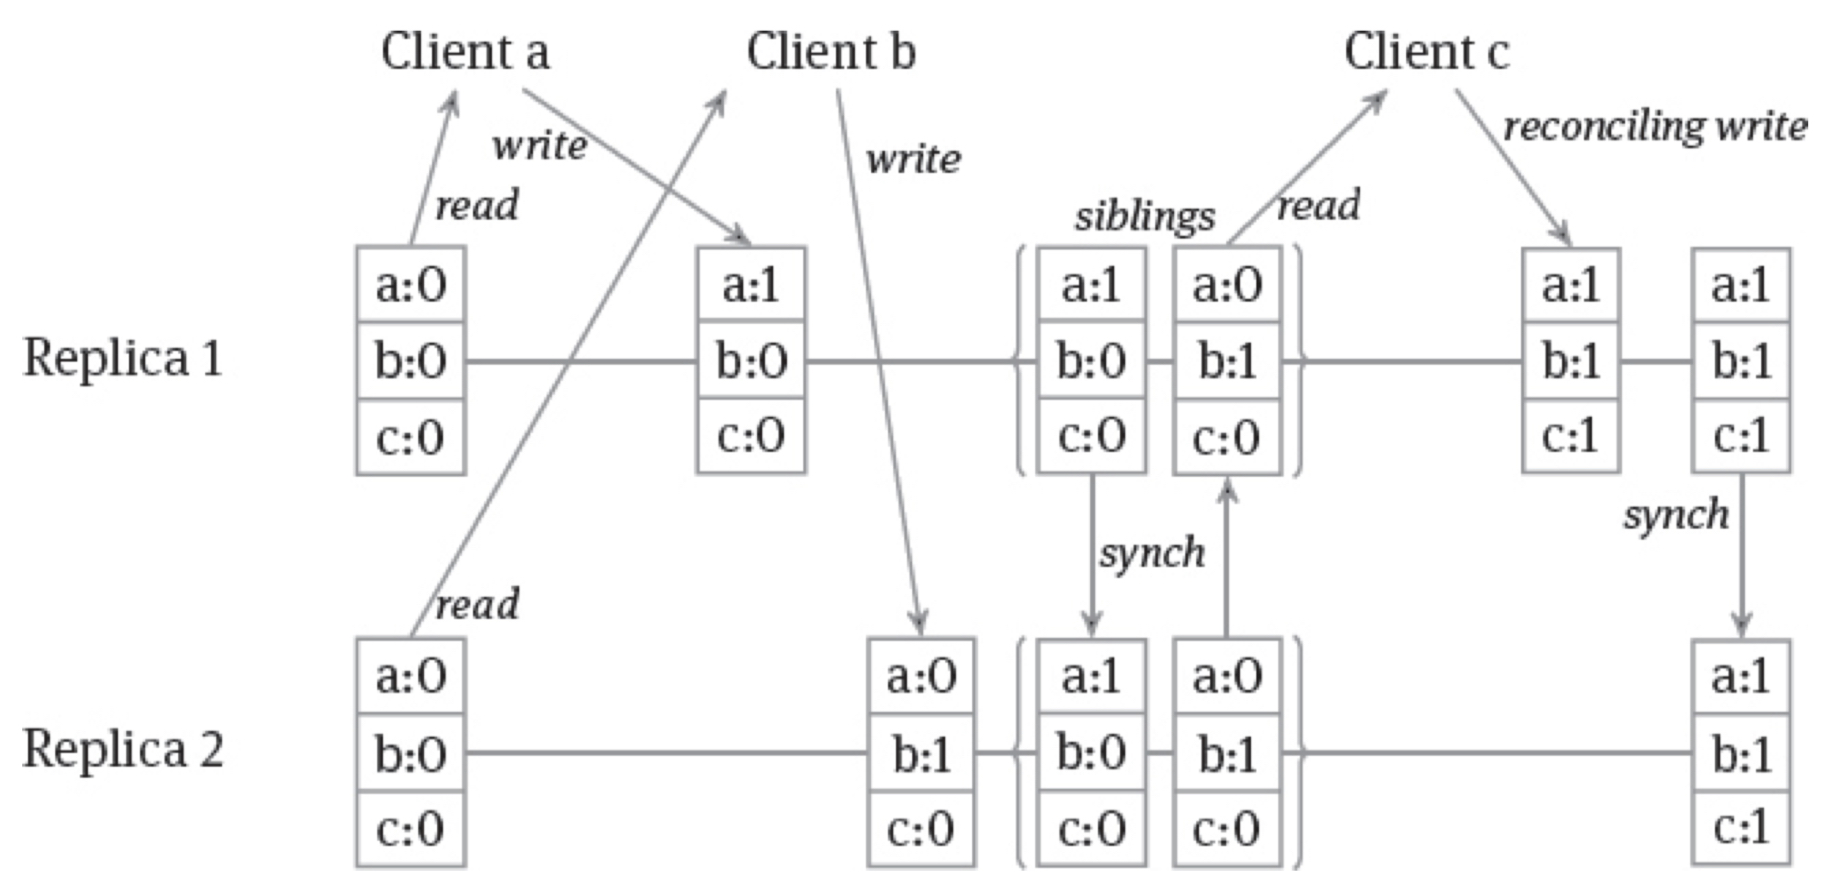
\includegraphics[width=.7\linewidth]{images/AdvancedDataManagment/distribute_concurrency_control/version_vector-siblings.jpeg}
\end{figure}

\section{Optimizations of Vector Clocks}
Distributed systems with vector clocks thus need some kind of \textbf{vector clock bounding} in order to support a large number of client processes over a long period of time.

\subsection{Client IDs versus replica IDs}
\begin{itemize}
    \item For version vectors, one way to reduce the size of the vectors is to use \textbf{replica IDs} instead of client IDs.
    \item This is based on the observation that synchronization takes place only between replicas and hence version vectors only need one element per replica for each data record
    \item However, with a simple counter for each of the replica IDs we run into the following problem of \textbf{lost updates}
    \item Two clients might concurrently write to the same replica based on an identical context
    \item With a version vector based on client IDs, the database could simply handle the stale write as concurrent
    \item However, with version vectors simply based on replica IDs, this concurrency cannot be expressed
\end{itemize}

%IMAGE